\documentclass[12pt,letterpaper,noanswers]{exam}
\usepackage[usenames,dvipsnames,svgnames,table]{xcolor}
\usepackage[margin=0.9in]{geometry}
\renewcommand{\familydefault}{\sfdefault}
\usepackage{multicol}
\pagestyle{head}
\header{AM 111 Class 09}{}{Interpolation, p.\thepage}
\runningheadrule
\headrule
\usepackage{siunitx}
\usepackage{graphicx} % more modern
\usepackage{amsmath} 
\usepackage{amssymb} 
\usepackage{hyperref}
\usepackage{tcolorbox}
\usepackage{enumitem}
\def\mbf{\mathbf}
\newcommand{\vc}[1]{\boldsymbol{#1}}
\def\dsst{\displaystyle}
\DeclareMathOperator*{\argmin}{arg\,min} % thin space, limits underneath in displays


\begin{document}
 \pdfpageheight 11in 
  \pdfpagewidth 8.5in

\noindent 

\section*{Preliminaries}

\begin{itemize}
\itemsep0pt
\item Problem set 04 is due on Friday at noon.
\item There will be a skill check in class during Class 10.  The problem info is below.
\item Find all OH on Canvas.
\item Quiz 01 is on Thursday Oct 12.  There is quiz info on canvas.
\end{itemize}



\noindent\textbf{Big picture}

Today: Algorithms for finding a curve that directly passes through data points.

\vspace{0.2cm}
\hrule
\vspace{0.2cm}

\noindent \textbf{Skill check practice}
 Consider the data points $(1,7)$, $(3, 5)$, $(4, 9)$.  Construct $L_{3,1}$, the Lagrange basis function of degree $2$ that is $1$ at $x_1 = 1$ and is $0$ at the other input values.



\vspace{0.2cm}
\hrule
\vspace{0.2cm}

\noindent \textbf{Skill check solution}
For zeros at $3$ and $4$, we have $(x-3)(x-4)$.  For the function to be $1$ at $x = 1$, we have $L_{3,1} = \dfrac{(x-3)(x-4)}{(1-3)(1-4)}$

\vspace{0.2cm}
\hrule
\vspace{0.2cm}


\section*{Interpolation}
\subsection*{Some applications}

\subsection*{Numerical integration}


\subsection*{Polynomial interpolation of data}

\begin{enumerate}
\item Consider the data points $(0,3), (1,2), (2,4)$.  What is the lowest degree polynomial that will interpolate these points?
\vspace{0.6in}

\item Consider the data points $(0,3), (0,2), (2,4)$.  Is an interpolating function possible?  Why not?
\vspace{0.6in}

\end{enumerate}

\subsection*{Monomial basis}

\begin{enumerate}[resume]
\item Recall that the matrix \[\left[\begin{array}{c c c c}
1 & x_1 & \hdots & x_1^{n-1} \\
\vdots & \vdots & & \vdots \\
1 & x_n & \hdots & x_n^{n-1}
\end{array}\right]\] is called a \textbf{Vandermonde} matrix.  

%\emph{You worked with Vandermonde matrices on problem set 02.} 

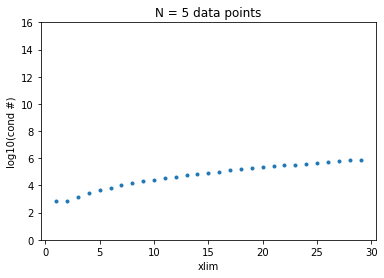
\includegraphics[width=0.45\textwidth]{img/Class08vandermonde5.png}
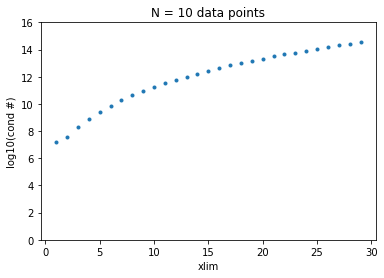
\includegraphics[width=0.45\textwidth]{img/Class08vandermonde10.png}

\begin{verbatim}
N = 5
xlim = 8
xlist = np.linspace(0,xlim,N)
A = np.vander(xlist)
condnum = np.linalg.cond(A)
\end{verbatim}

What makes the basis $1$, $x$, ..., $x^k$,..., $x^{N-1}$ a poor choice for finding an interpolating polynomial?
\vspace{1in}
\end{enumerate}



\noindent\textbf{Advantages of the monomial basis}


\subsection*{Lagrange interpolation}

\begin{enumerate}[resume]

\item Given two distinct points $(x_0,y_0)$ and $(x_1,y_1)$, find an equation for the
straight line through both points. 

Call this function $P(x)$.  Is it unique?

\emph{A line is the lowest dimensional interpolating polynomial for two points.}

\vspace{1in}

\item Show that the function $\dsst{L_0(x) = \frac{x-x_1}{x_0-x_1}}$ is $1$
when $x=x_0$ and $0$ when $x=x_1$.  

Similarly $\dsst{L_1(x) = \frac{x-x_0}{x_1-x_0}}$
is $0$ when $x=x_0$ and $1$ when $x=x_1$.

\vspace{1in}

\item Consider the function $Q(x) = y_0L_0(x) + y_1L_1(x)$.  Show that it is
equal to $P(x)$.

\vspace{1in}

\end{enumerate}


\begin{enumerate}[resume]

\item Construct the Lagrange interpolating polynomial that goes through the points $(0,1)$, $(2,2)$, and $(3,4)$.  %Simplify it to the form $P(x) = ax^2 + bx + c$.

\vspace{1in}

\item Consider the Lagrange interpolation problem.  If it is written in the form $A\vc{c} = \vc{y}$ (where $\mathbf{c}$ are the weights assigned to the basis functions), what is the structure of $A$?

\emph{Use your knowledge of the values of the weights, $\vc{c}$.}
\vspace{0.5in}
\end{enumerate}


\subsection*{Newton's divided differences}



\begin{enumerate}[resume]
\item For $(0,1), (2,3)$ construct $A\mathbf{c} = \mathbf{y}$ or the divided difference table.



Let $P_1(x) = c_0 + c_1(x-0)$.  Find $c_0$ and $c_1$.

Check $P_1(0)$ and $P_1(2)$.

\vspace{2in}

\item Add the third data point $(3,0)$.

$P(x) = c_0 + c_1(x-0) + c_2(x-0)(x-2)$.  Find $c_0$, $c_1$, $c_2$.

Check $P(0), P(2)$, and $P(3)$.
\end{enumerate}


\end{document}